\chapter{Trending}\label{trend}

We look at trends on twitter and in finance and try to see if there are any
correlations between them. Before we got into the trends we made some
assumptions to set the trend context.  

The Norwegian stock exchange, OSEBX, is largely an oil based exchange. And
therefore we assume that oil related data will give a good indications of the
behavior of OSEBX. Section \ref{data:trend_data} says something about why we
choose tweets based on oil for the trend aggregation.

Further we wanted to look at trading that is not algorithm based, also
known as speed trading. So we started looking at technical analysis. The
technical analysis gives a base for decision support for the trader. The
techniques of technical analysis gives us good indications about trends, but we
want to take it further by involving sentiment. 

We start of by describing and defining a trend in section
\ref{trend:trend_is_your_friend}. Continuing with trends on an in relation to
twitter, \ref{trend:trends_on_twitter}. To be followed by trends in finance,
\ref{trend:trends_in_finance}. An last we Compare twitter trends with finance
trends, \ref{trend:compared}.
%

\section{The trend is your friend}\label{trend:trend_is_your_friend}
A trend is a series of changes that moves in the same direction over a period
of time. It is often associated with fashion or stock trading. The
definition of trend is "the general course or prevailing
tendency"\footnote{Dictionary.com:
\url{http://dictionary.referencs.com/browse/trend}}.

In finance especially the trend can be a deciding factor in buying or selling
of goods. You typically do not want to sell during a bullish trend, while the
value is going up. And you want to sell before you get to the bearish trend,
when the value goes down. Figure \ref{fig:stocktrends} shows basic trends on
page \pageref{fig:stocktrends}. When markets do not trend they move sideways in
trading ranges\footnote{Swing-trade-stocks.com \url{http://www.swing-trade-stocks.com/stock-trends.html}}.  

\begin{figure}[htb]
    \centering
    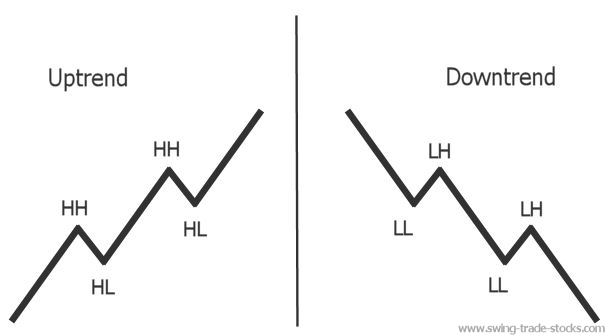
\includegraphics[width=\textwidth]{stocktrends.jpg} 
    \label{fig:stocktrends}
    \caption{Basic trend}
Showing Higher Highs(HH), Lower Highs(LH), Higher Lows(HL), and Lower Lows(LL). 
\end{figure}

Average directional Index Indicator, ADX, gives clear, easy-to-read picture of
the market, shown in figure \ref{fig:ADX-Example-Stock-Trading} on page
\pageref{fig:ADX-Example-Stock-Trading}. It shows if the trend strengthens of
weakens. Moving averages and parabolic SAR can help to confirm a move or
determine a trend. Moving averages indicates change over a period of time. The
time frame is adjusted to the time the trader likes to keep stocks. The
parabolic SAR looks at the price of a stock and determines the trend as upwards
or downwards. When upwards the plotted dots are below the price, and vice versa.
 
\begin{figure}[htb]
    \centering
    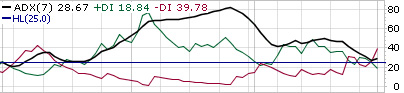
\includegraphics[width=\textwidth]{ADX-Example-Stock-Trading.jpg} 
    \label{fig:ADX-Example-Stock-Trading}
    \caption{Average Directional Index example}
An example of ADX. Green line is showing increase in price. Red line is
decrease. The black line is the ADX. 
\end{figure}

When using ADX or other trend tools it is difficult to spot the trend or at all
predict it. The ADX graph has some indicators of trends. The further away from
each other the red and green lines are, the stronger the trend is.  
When trading based on the trend, the problem is to find the trend and predict
it into the future. And this is where we combine Twitter with traditional
trading. If we could predict the trend based on public opinion mined from
twitter we would have an advantage. 

Data is increasingly important for trend prediction. The better data we have,
the better trend we can predict. By focusing on sentiment we aim for the
cooperation of information available on the Internet and the value of sentiment
to predict trends. This will be more important in the future.  

If the trend is your friend, you know how the market will move and make
good decisions in accordance with the trend. 
%

\section{Trending in Finance}\label{trend:trends_in_finance}
The average directional index and the moving average techniques for trend
calculation is described.  

\paragraph{Moving Average(MA)}
\hspace{0pt}\\
MA is the unweighted mean of the previous n days.
Given the closing price of the last n days as:

\math{
p_M, p_{M-1},\dots,p_{M-(n-1)}
}\\

We have that the simple moving average is : 

\math{
\textit{SMA} = { p_M + p_{M-1} + \cdots + p_{M-(n-1)} \over n }
}\\

There are also other variants of the moving average. Such as cumulative MA,
weighted MA and exponential MA\footnote{Wikipedia:
\url{https://en.wikipedia.org/wiki/Moving_average}}. 

\paragraph{ADX}
\hspace{0pt}\\
ADX\footnote{Wikipedia:
\url{https://en.wikipedia.org/wiki/Average_Directional_Index}} uses the positive directional indicator(+DI) and the negative directional
indicator(-DI) in combination to determine a trend. The high, low and closing
values are needed for the ADX to be calculated. The directional movement is
calculated as follows: 

\begin{verbatim}
UpMove = today's high − yesterday's high
DownMove = yesterday's low − today's low
if UpMove > DownMove and UpMove > 0, then +DM = UpMove, else +DM = 0
if DownMove > UpMove and DownMove > 0, then −DM = DownMove, else −DM = 0 
\end{verbatim} 

When the directions are calculated we choose the time frame we want to
investigate. And get -DI and +DI:

\begin{verbatim}
+DI = 100 times exponential moving average of +DM 
      divided by average true range
-DI = 100 times exponential moving average of −DM 
      divided by average true range 
\end{verbatim} 

Where the time frame defines the number of periods used in the exponential
moving average. And the average true is an exponential average of the true
range. Resulting in the ADX:

\begin{verbatim}
ADX = 100 times the exponential moving average 
      of the absolute value of (+DI − −DI) 
      divided by (+DI + −DI)
\end{verbatim}

\paragraph{Experiments}
\hspace{0pt}\\
In the experiment, section \ref{experiments:trend} on page
\pageref{experiments:trend} we plot the graph and look at coding details for
the finance trends. In the experiment we used data from the Oslo stock exchange
in the same period as we took tweets, Apr 26 - May 26.
%

\section{Trends from Twitter}\label{trend:trends_on_twitter}
There are two parts to trends with twitter. The trends Twitter themselves
create based on words of hashtags that appear in many tweets. And the trend we
compile ourselves based on the trend data described in section
\ref{data:trend_data}, page \pageref{data:trend_data}. 

\paragraph{On Twitter}
\hspace{0pt}\\
On Twitter there is a feature called 'Trends'. It shows the words that are used
the most lately. A screen capture of it can be seen in figure
\ref{fig:trends_on_twitter}, on page \pageref{fig:trends_on_twitter}.
\begin{figure}[htb]
	\centering
    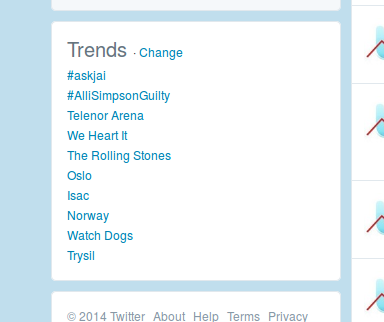
\includegraphics[width=0.5\textwidth]{trends_on_twitter.png}
    \label{fig:trends_on_twitter}
    \caption{Trends on Twitter}
Screen capture from Twitter.
\end{figure}

The trends on twitter are in many cases predictable and adds little value to trend
compilation. The trend on twitter is also specialised for each user, based on
that users subscriptions and location. As an example at the Norwegian national
day(Mai 17.) we would have trending words like \texti{Norge}, \textit{Norway},
and \textit{#17Mai}. Today we already know that this will happen again next year. 
%

\paragraph{Our own}
\hspace{0pt}\\
Using the trend data described in section \ref{data:trend_data} we construct a
moving average graph and a ADX graph. 

The referenced article lists the most important oil related account on twitter.
In two parts. One for the Norwegian ones, and one for international ones. 
To simplify the trend creation a bit we used mostly English tweets, ignoring
most of the Norwegian twitter handles. 

After sorting the mined tweets by day we classify all tweets for each day. The
classification from each day is referred to as a trend day. The trend day
contains the amount of positive tweets, the amount of negative tweets, and the
total amount of tweets.

\begin{python}
trend_days = {
	'trend-Apr-30': {'neg': 112, 'pos': 131, 'tot': 243},
    'trend-May-19': {'neg': 523, 'pos': 1326, 'tot': 1849},
    'trend-May-18': {'neg': 59, 'pos': 110, 'tot': 169},
    'trend-May-15': {'neg': 1151, 'pos': 2255, 'tot': 3406},
}
\end{python}  

Now we have some sentiment data to create a trend from. To simplify the trend
aggregation and the graph plotting, we transform the data to fit into the
format used for the finance data.  

\begin{verbatim}
Date,close,high,low,open,volume
20140423,559.41,562.45,557.74,561.13,0
20140424,562.89,565.65,559.84,559.41,0
20140425,566.24,566.24,562.41,562.89,0
20140428,566.82,567.14,564.55,566.24,0
\end{verbatim}

To transform the data we do the following: 
\begin{python}
trend_days = get_tweet_trend_data()
keys = sorted(trend_days.keys())
date = ""
for i in range(1, len(keys)):
    if "Apr" in keys[i]:
        date = "201404" + str(keys[i].split('-')[2])
    elif "May" in keys[i]:
        date = "201405" + str(keys[i].split('-')[2])
    volume = trend_days[keys[i]]['tot'] * 1.0
    # (positive_tweets / total_amount_of_tweets)*scale
    high = (trend_days[keys[i]]['pos'] / volume) * 1000
    # (negative_teets / total_amount_of_tweets)*scale
    low = (trend_days[keys[i]]['neg'] / volume) * 1000
    openv = 0
    close = high - low
    print str(date) + "," + str(close) + "," + str(high) \
          + str(",") +str(low) + "," + str(volume / 10) + \
          "," + str(0)
\end{python}

We scale the values to plot a more representative graph. All the
proportions are kept intact, so the moving average and ADX is still valid.
This method is tested in section \ref{experiments:trend} on page
\pageref{experiments:trend}.
% 

\section{Comparing the trends}\label{trend:compared}
Comparing the finance trend and the Twitter based trend is easy. We look at the
two graphs and draw conclusions. Drawing the conclusions are the difficult
part.

We look at the two plotted trends, the moving average and the average direction
index. More specifically we compare the white MA of both graphs with each other
to. And the blue MA lines of each graph with each other. 

With the ADX we will look for similar movements and turning points for the
graphs. Also areas where the red and green graphs stay separate. 

Further comparison should give some conclusions of the trust worthiness of the
sentiment trend. For traders to trust in the sentiment as a new way of
predicting trends the sentiment would have to provide profit and scientifically
proven results. At this stage there would be few who would rely on sentiment as
a predictor of trends.
The trust lies in the technical analysis.  

With the comparison we have the drawback of examining a stock exchange instead
of one stock. Comparing one stock at a time would give better indications of
the accuracy of the sentiment trend. This should be explored further in the
future.   
%

\section{Future work}
For future improvements of the trend aggregation we should into three aspects.
The Norwegian market we started with, and explore the oil tweets. And find out
whether or not they are a good indication of the OSEBX. 

And we should look into single stocks in the comparison of trends. This way we
can explore the stock vs stock Twitter trends, and find new information there.  
%
